% This starts the document; the "npsreport2018" style is really a modified report style. 
\documentclass[techreport, article]{npsreport2018}
\frenchspacing


% Put extra packages you may need to customize 
%\usepackage[fontsize=20pt,text=To~be~replaced~by~your~thesis~processor~using~the~data~from~your~Python~Thesis~Dashboard,color=red]{draftwatermark}
\usepackage[bottom]{footmisc} % Places footnotes at the bottom of the page

\usepackage{url}
%\usepackage{hyperref}
%\usepackage{fancyhdr}
%\usepackage{graphicx}
%\usepackage{tabularx}
%\usepackage{enumitem}
%\usepackage{indentfirst}
%\usepackage{subcaption}
%\usepackage{amsmath, amssymb}
\usepackage{units}
\usepackage{IEEEtrantools}

\title{Applying Spectral Representation to Simulation of Stochastic Processes: Scaling, Units, Sidedness}

\author{Brian Bingham}
\rank{Professor, Mechanical and Aerospace Engineering Department}  
\degreedate{1 April 2023}

% Match to your thesis dashboard
\distribution{Approved for public release. Distribution is unlimited.}

% Paste abstract from your thesis dashboard. New paragraphs start after an empty line.
\abstract{
Simulation provides a virtual environment to support development engineering system through test and evaluation in variety of environmental conditions. In order to provide quantitative results, the simulated environmental conditions must be derived from accurate descriptions of the physical environment, which are often described as stochastic processes.   For example, authentic synthetic wind and wave environments are an important part of evaluating ship designs.  For these sythetic environments to accurately represent they physical operating environment they must be statistically consistent with the cooresponding oceanographic and meteorological stochastic descriptions.
\\ \\Because physical environments are often described as stocastic processes and defined by power spectral density functions, generating physically meaningful sythetic environments requires generating sample functions of the underlying power spectra.  While the relationship between a spectral description and a time series sampled from that description is mathematically well defined, applying these methods to generate physical processes requires attention to the details of spectra normalization scaling, engineering unit conventions and sidedness of the spectral representation.  
\\ \\This report synthesizes the basic mathematical background, presented with the intent of providing a self-consistent set of conventions for the practitioner.  Two common methods for time series generate are described, summation of cosines and fast Fourier transforms along with a complete example in MATLAB to illustrate the important details of considering scaling, units and sidedness.
}

% If CUI (Controlled Unclassified Information)
\securitybanner{}  %\securitybanner{CUI}, remove when requesting FINAL REVIEW with thesis processor, who will insert final banners.
%
%Do NOT upload CUI to websites like Overleaf
%

%
% Mandatory fields for the SF298.
%
\ReportType{Technical}
\ReportDate{1 April 2023}       % for a thesis, graduation date
\SponsoringAgency{Naval Postgraduate School \\ Monterey, CA 93943}   
\DatesCovered{1 JAN 2023 to 1 APR 2023}
\ReportClassification{U}
\AbstractClassification{U}
\PageClassification{U}
%
% Optional fields for the SF298.
%
\RPTpreparedFor{Naval Postgraduate School}
\ContractNumber{}
\GrantNumber{}
\ProgramElementNumber{}
\TaskNumber{}
\WorkUnitNumber{}
\POReportNumber{NPS-MAE-23-002}
\Acronyms{}
\SMReportNumber{}
\SubjectTerms{timeseries, stocastic processes, simulation, spectral representation, wave generation}
\ResponsiblePerson{Brian Bingham}
\RPTelephone{(831) 200-6360}
\SignatureOne{}
\SignatureTwo{}
\SupplementaryNotes{The views expressed in this document are those of the author and do not reflect the official policy or position of the Department of Defense or the U.S. Government.
}

% Optional. Prevents footnotes from being reset at each chapter
% Comment this out to have them reset with each chapter.
\makeatletter
\@removefromreset{footnote}{chapter}
\makeatother

% Optional. Adds pdf metadata and links.
% This should be right before the \begin{document}, to be the
% last package / macros defined. (Hyper-ref is fragile,
% needs to be last, and has known conflicts with other packages.)
% Comment out if you have build problems building with hyperref
\NPShyperref

% For signature page
\researchchair{Kevin A. Smith}
\departmentchair{Jomana Amara}
\department{Vice Provost of Academic Leadership}
\SponsoringNotation{}
%
% Your thesis begins here
%
\begin{document}
%% IEEE format only and Mechanical and Aerospace Engineering (MAE) Department only:
%% Uncomment the next line.  All others, leave commented out (with % sign)
%\bstctlcite{forced-et-al-off}
\NPScover                  % Cover page
\NPSsftne                  % SF298 form
\NPSsignature             % Tech Report page (iii): signature page
%\NPSthesistitle            % Thesis page (iii): title page
\NPSabstractpage           % Abstract Page
%\NPSfrontmatter            % NPS front matter follows
%\DraftwatermarkOptions{stamp=false} % Starting at this point in the document, this commands the draftwatermark package to stop printing.
% set the figure default size
\newcommand{\SF}{0.8}
\newcommand{\SFb}{0.45}
\newcommand{\SFPic}{0.45}
\newcommand{\SFPlot}{0.45}
\newcommand{\SFc}{0.52}
% Just a lazy way of setting the figure width (percentage of text width)
% 0.7 works well for 1 column
% 0.4 works well for 2 column
\newcommand{\FigWidth}{\SF}


%
% If you don't need one of these, comment it out.
%
%\setcounter{page}{7} % -- if you need to change the page number for the TOC do it here
%\NPStableOfContents
%\NPSlistOfFigures
%\NPSlistOfTables
%\NPSlistOfAcronymsFromFile{acronyms}

% Acronyms
\acrodef{psd}[PSD]{power spectral density}


% Start layout for the NPS body
\NPSbody

\section{Introduction}
Many of the environmental influences on an engineered system can be modeled as stochastic processes where the particular environmental conditions are described by the \ac{psd} of the process.  For maritime vessels, waves and wind have important influences on control and perception.  Using spectral representations of these influences improves the connection between the simulated environment and field conditions.  This study is motivated by our recent work in simulation of environmental influences upon ocean robotic systems at and below the water surface \cite{bingham2019maritime, zhang22dave, choi22fasterrohtua}.

As pointed out in \cite{barbour15normalization} the variety of nomenclature, conventions and definitions in spectral analysis leads to considerable confusion and often improper use when applying these techniques.

This article describes techniques to generate a time series, $y(t)$, that is a sample function (a realization) of the one dimensional, univariate (1D-1V) stochastic process, $y_o(t)$, with a given one-sided \ac{psd} function $S_{y_{o}}(\omega)$, where $\omega$ is angular frequency in \unit[]{rad/s}.  %We present techniques based on \emph{spectral representation methods}.
Methods for simulation of stochastic process include covariance decomposition, auto-regressive moving-average (ARMA), noise shower, scale refinement, turning band and spectral representation \cite{cao00simulation}.  This report discusses the spectral representation method.


\subsection{Background}
Foundational work on spectral representation of a stochastic process was done by 
 Rice \cite{rice44mathematical1,rice45mathematical2}.  Some of the original approaches to generating a time series with given \ac{psd} were based the design of a linear filter for which white noise input would generate an output with the desired \ac{psd}.  Introduced sum of cosines \cite{borgman69ocean, shinozuka72monte}.  The methods covered in this report include the following:
\begin{itemize}
\item Linear filtering and spectral factorization.
\item Spectral representation - sum of cosines
\item Spectral representation - FFT/IFFT
\end{itemize}
\noindent
For general time series analysis see \cite{marchal15notes} and the references therein.

\subsection{Frequency, Sidedness, Conventions, Notation and Scaling}

Our goal is to generate time series realizations of stochastic processes described by spectral representations.  Spectral representation is a concise way to describe a physical phenomena (wave, wind, etc.) based on thorough empirical analysis, allowing the simulated time series to embody authentic physical scenarios.  Because of this connection between the spectral representation and the time series, it is important to address the following issues:
\begin{itemize}
\item Expression of the frequency variable in angular or oscillation frequency.
\item Scaling of the Fourier transform and Fourier series resulting from the choice of frequency units.
\item Use of the two-sided or one-sided \ac{psd}.
\end{itemize}
Often the details of the conventions used are ambiguous because these issues are not of primary importance in mathematics and physics domains, or in applications where both the transform and inverse transform are used.  However, for our engineering applications, maintaining the physical relevance between the expression of the \ac{psd} (in either frequency units and either sidedness) and the time series with physically meaningful units is important for the purposes of generating environmental influences that are statistically representative of the underlying spectral descriptions.  The contribution of this report is to provide a complete and consistent synthesis of the simulation generation process with explicit notation to make use of the various conventions for expressing \ac{psd} sidedness, frequency units and Fourier transform scaling.


\section{Preliminaries}

\subsection{Integration by Substitution}

Given the functional relation $u=\phi(x)$, the following is true for finite, single variable integrals\footnote{\url{https://en.wikipedia.org/wiki/Integration_by_substitution}}:
\begin{equation}
  \int_{\varphi(a)}^{\varphi(b)} y(u) du = \int_a^b y(\varphi(x)) \left(\frac{d \varphi(x)}{dx}\right) dx.
  \label{e:ibs}
\end{equation}
This will be useful when changing variables, e.g., between oscillation and angular frequency.

\subsection{Fourier Transform}

\subsubsection{Oscillation Frequency: $\unit[f]{[Hz]}$}

When using the oscillation frequency in Hertz, the continuous time Fourier and inverse Fourier transform exhibit symmetry
\begin{IEEEeqnarray}{rClCl}
  \IEEEyesnumber\label{e:fo} \IEEEyessubnumber*
  X(f) & = & \int_{-\infty}^{\infty}x(t)e^{-j (2 \pi f) t}dt & = & \mathcal{F}\{x(t)\} \\
  x(t) & = & \int_{-\infty}^{\infty}X(f)e^{j (2 \pi f) t}df & = & \mathcal{F}^{-1}\{X(f)\}
\end{IEEEeqnarray}
where we use the notation $\mathcal{F}{\cdot}$ for the Fourier transform operator and $\mathcal{F}^{-1}{\cdot}$ for the inverse Fourier transform operator.

\subsubsection{Angular Frequency: $\unit[\omega]{[rad/s]}$}
However, expressing the transforms in terms of angular frequency, $\omega = 2 \pi f$, destroys this symmetry\footnote{\url{http://mathworld.wolfram.com/FourierTransform.html}}.  To make matters worse, there are a variety of conventions when it comes to writing the definition of the transform with angular frequency, hence the ``plethora of rival conventions of the definition of the Fourier transform''\footnote{\url{https://en.wikipedia.org/wiki/Fourier_transform\#Units_and_duality}}. If we use integration by substitution (\ref{e:ibs}) and the definition (\ref{e:fo}) results in 
\begin{IEEEeqnarray}{rCl}
  X(\omega) & = & \int_{-\infty}^{\infty}x(t)e^{-j \omega t}dt \\
  x(t) & = & \frac{1}{2 \pi} \int_{-\infty}^{\infty}X(\omega)e^{j \omega t}d\omega
\end{IEEEeqnarray}
We can also write the transform pair as
\begin{IEEEeqnarray}{rCl}
  X_2(\omega) & = & \frac{1}{\sqrt{2 \pi}} \int_{-\infty}^{\infty}x(t)e^{-j \omega t}dt \\
  x(t) & = & \frac{1}{\sqrt{2 \pi}} \int_{-\infty}^{\infty}X_2(\omega)e^{j \omega t}d\omega
\end{IEEEeqnarray}
which is similar to the Fourier-Stieltjes transform used commonly in probability theory.  Another possible convention is
\begin{IEEEeqnarray}{rCl}
  X_3(\omega) & = & \frac{1}{2 \pi} \int_{-\infty}^{\infty}x(t)e^{-j \omega t}dt \\
  x(t) & = & \int_{-\infty}^{\infty}X_3(\omega)e^{j \omega t}d\omega
\end{IEEEeqnarray}


\subsubsection{Einstein-Wiener-Khinchin Theorem}
The theorem states that,  ``the autocorrelation function of a wide-sense-stationary random process has a spectral decomposition given by the power spectrum of that process''\footnote{\url{https://en.wikipedia.org/wiki/Wiener-Khinchin_theorem}}.


Consider a zero-mean, real-valued, wide-sense stationary\footnote{Wide-sense stationarity is a weaker form of strict sense stationarity.  For a wide-sense stationary stochastic process the mean and the autocorrelation are time invariant - and the energy is finite.} $x(t)$.  The autocorrelation is defined as
\[
R_{xx}(\tau) = E[x(t+\tau)x(t)] 
\]
where $E(\cdot)$ is the expectation operator. Under reasonable assumptions of continuity and differentiability, the autocorrelation and \ac{psd} are Fourier transform pairs.  In units of oscillation frequency this is expressed as
\begin{IEEEeqnarray}{rClCl}
  \IEEEyesnumber\label{e:ewkf} \IEEEyessubnumber*
  S_{xx}(f) & = & \int_{-\infty}^{\infty}R_{xx}(\tau)e^{-j (2 \pi f) \tau}d\tau & = & \mathcal{F}\{R_{xx}(\tau)\} \\
  R_{xx}(\tau) & = & \int_{-\infty}^{\infty}S_{xx}(f)e^{j (2 \pi f) \tau}df & = & \mathcal{F}^{-1}\{S_{xx}(f)\}
\end{IEEEeqnarray}

It is important to note $S_{xx}(f)$ refers to the {\bf two-sided} \ac{psd}.  For real-valued processes, the \ac{psd} is symmetric about $f=0$, i.e., $S_{xx}(f) = S_{xx}(-f)$.  Often times the {\bf one-sided} \ac{psd}, $\Sigma_{xx}(f)$    is used for just positive frequencies.  The two are related by
\begin{equation}
  \Sigma_{xx}(f) = 2 \, S_{xx}(f), \; \forall f \geq 0,
  \label{e:onetwo}
\end{equation}
and the integrals involving the one-sided spectrum have a lower limit of $0$ rather than $-\infty$.

This relation allows us to illustrate the relation between \ac{psd} and power. The expected power in the process $x(t)$, equivalent to the variance of the process ($\sigma^2$), is
\begin{IEEEeqnarray}{rClClCl}
  \IEEEyesnumber\label{e:psd} \IEEEyessubnumber*
  E[x^2(t)] & = & \sigma^2 & = & R_{xx}(\tau=0) & = & \int_{-\infty}^{\infty}S_{xx}(f)e^{j (2 \pi f) (\tau=0)}df \\
  & & & & & = & \int_{-\infty}^{\infty}S_{xx}(f) df \\
  & & & & & = & 2 \int_{0}^{\infty}S_{xx}(f) df \\
  & & & & & = & \int_{0}^{\infty}\Sigma_{xx}(f) df
\end{IEEEeqnarray}
which is the area under the \ac{psd} curve.

\subsubsection{Power Spectral Density and Angular Frequency}
Expressing the \ac{psd} in angular frequency ($\unit[\omega]{[rad/s]}$) can be error prone.  We define the two-sided \ac{psd} in angular frequency as a separate function, $G_{xx}(\omega)$.  This expression must also be consistent with the expected power relationships (\ref{e:psd}), so using the integration by substitution (\ref{e:ibs}) we find
\begin{IEEEeqnarray}{rClCl}
  \IEEEyesnumber\label{e:psdw} \IEEEyessubnumber*
  E[x^2(t)] & = & R_{xx}(\tau=0) & = & \int_{-\infty}^{\infty}S_{xx}(f) df \\
  & & & = &  \int_{-\infty}^{\infty}S_{xx}(f = \omega/(2 \pi)) \left( \frac{df}{d\omega}\right) d\omega \\
   & & & = & \frac{1}{2\pi} \int_{-\infty}^{\infty}S_{xx}(f = \omega/(2 \pi)) d\omega \\
  & & & = & \frac{1}{\pi} \int_{0}^{\infty}S_{xx}(f=\omega/(2 \pi)) d\omega \\
  & & & = & \frac{1}{2\pi}  \int_{0}^{\infty}\Sigma_{xx}(f=\omega/(2\pi)) d\omega .
\end{IEEEeqnarray}
Equations (\ref{e:psdw}) are applicable when provided with a \ac{psd} function expressed in oscillation frequency, but carrying out the integration in angular frequency.  If the \ac{psd} is expressed in angular frequency, the intention may be that
\begin{equation}
  G_{xx}(\omega) = \frac{1}{2 \pi} S_{xx}(f = \omega/(2 \pi)
\end{equation}
where $G_{xx}(\omega)$ is the two-sided \ac{psd} in angular frequency and the corresponding one-sided \ac{psd} in angular frequency is
\begin{equation}
  \Gamma_{xx}(\omega) = 2 G_{xx}(\omega) = \frac{1}{\pi} S_{xx}(f=\omega/(2\pi) = \frac{1}{2 pi} \Sigma_{xx}(f=\omega/(2\pi), \; \forall \omega \geq 0,
  \label{e:onetwow}
\end{equation}
which implies that
\begin{IEEEeqnarray}{rClCl}
  \IEEEyesnumber\label{e:psdw2} \IEEEyessubnumber*
  E[x^2(t)] & = & R_{xx}(\tau=0) & = & \int_{-\infty}^{\infty}G_{xx}(\omega) d\omega \\
  & & & = & 2 \int_{0}^{\infty}G_{xx}(\omega) d\omega \\
  & & & = & \int_{0}^{\infty}\Gamma_{xx}(\omega) d\omega .
\end{IEEEeqnarray}


\section{Generating Time Series}

\subsection{Summation of Cosines Method}

Using the explicit notation above, the simulation formula from \cite{shinozuka91simulation} can be applied to generate the time series $y^{(i)}(t)$ that is the $i$-th realization of the stochastic process $y(t)$ described by the two-sided \ac{psd} $G_{yy}(\omega)$ expressed in angular frequency.  This simulation formula converges to the series as $N \rightarrow \infty$:
\begin{equation}
  y^{(i)}(t) = \sqrt{2} \sum_{n=0}^{N-1} A_n \cos(\omega_n t + \phi^{(i)}_n)
  \label{e:sumcosines}
\end{equation}
where
\begin{IEEEeqnarray}{C}
\IEEEyesnumber\label{e:sim} \IEEEyessubnumber*
A_n = (2 \, G_{yy}(\omega_n)\Delta \omega)^{1/2},  \;  n=0,1,2,...,N-1 \label{e:an} \\
\omega_n = n \Delta \omega, \; n=0,1,2,...,N-1 \label{e:lrs}\\
\Delta \omega = \omega_u / N.
\end{IEEEeqnarray}
The frequency sampling is $\Delta\omega$, the upper cut-off frequency, $\omega_u$, is the frequency beyond which the \ac{psd} may be assumed to be zero, $\phi^{(i)}_0, \phi^{(i)}_1, ... , \phi^{(i)}_{N-1}$ are the $i$-th realizations of random phase angles distributed uniformly over the interval $[0,2\pi)$
and to avoid aliasing the time step (sampling time) is constrained by
\begin{IEEEeqnarray}{rCl}
\IEEEyesnumber\label{e:deltat} \IEEEyessubnumber*
\Delta t & \leq & \frac{2 \pi}{ 2 \omega_u} = \frac{\pi}{\omega_u}\\
& \leq & \frac{1}{2} \left( \frac{2 \pi}{\Delta \omega} \right) \frac{1}{N} = 
\frac{\pi}{\Delta \omega \, N}\\
& \leq & \frac{1}{2} \left( \frac{1}{\Delta f} \right) \frac{1}{N} = \frac{1}{2 \, \Delta f \, N}
\end{IEEEeqnarray}
with the sampling frequency expressed as both angular and oscillation frequencies. The condition
\begin{equation}
  A_0 = 0 \; \mathrm{or} \; G_{yy}(\omega_0=0)=0
  \label{e:an0}
\end{equation}
is necessary and must be forced if $G_{yy}(0)\neq 0$.  The simulated time series is periodic with period
\begin{equation}
  \label{e:T0}
  T_0 = \frac{2\pi}{\Delta \omega}.
\end{equation}

\subsubsection{Periodicity, Simulation Error and Convergence}

By examining the error between the time series ensemble autocorrelation and the
desired autocorrelation is proportional we can quantify the quality of the time series reproduction of the target \ac{psd}. In \cite{shinozuka91simulation} the authors show, using \cite{conte17elementary},  that for the simulation equations (\ref{e:sumcosines}) and (\ref{e:sim}) the rate of convergence proportional to $1/N$.It is worth noting that the frequency sampling (\ref{e:lrs}) of the summation in (\ref{e:sumcosines}) is analogous to integral approximation by a left Riemann sum, which is consistent with an error function that decreases with $1/N$.

An alternative approach is to use frequency sampling analogous to a middle Riemann sum method by sampling of the spectrum according to 
\begin{equation}
  \omega_n = n \Delta \omega + \Delta \omega /2 , \; n=0,1,2,...,N-1
  \label{e:mrs}
\end{equation}
instead of (\ref{e:lrs}).
The analogy holds that as would be expected for a middle Riemann sum, the convergence when using (\ref{e:mrs}) is proportional to $1/N^2$.  Also the periodicity of the resulting time series is doubled to
\begin{equation}
  T_o = 4\pi / \Delta \omega.
  \label{e:to}
\end{equation}
A disadvantage of this approach is that it cannot be implemented with the FFT technique below.

Note that \cite{hu97simulation} present a slight modification of the summation of cosines formulation that converges on the order of $1/N^4$.  The modification only affects the first two terms.

\subsection{Fast Fourier Transform (FFT) Method}
The FFT algorithm can be applied to the summation in (\ref{e:sumcosines}) to improve the computational efficiency of generating the complete sample function at once \cite{yang72simulation}.
The discrete-time Fourier series (DTFS) for finite series\footnote{\url{https://www.princeton.edu/~cuff/ele201/kulkarni_text/frequency.pdf} and \url{https://web.eecs.umich.edu/~fessler/course/451/l/pdf/c5.pdf}} is defined by the forward and inverse transform pair
\begin{IEEEeqnarray}{rCl}
  \IEEEyesnumber\label{e:dft} \IEEEyessubnumber*
  X[k] & = & \sum_{m=0}^{M-1} x[n] e^{-j \left(\frac{2 \pi}{M}\right) k \, n} \label{e:fft}\\
  x[n] & = & \frac{1}{M} \sum_{k=0}^{M-1} X[k] e^{j \left(\frac{2 \pi}{M}\right) k \, n} \label{e:idtfs}
\end{IEEEeqnarray}
for a time series $x[n]$ and a frequency series $X[k]$ of length $M$
\begin{IEEEeqnarray}{rll}
  \IEEEyesnumber\label{e:series} \IEEEyessubnumber*
  x[n] & : \; & n = 0, 1, ..., M-1 \\
  X[k] & : \; & k = 0, 1, ..., M-1.
\end{IEEEeqnarray}


To make use of the computation efficiency of the FFT technique, the summation of cosines simulation formula (\ref{e:sumcosines}), with frequency sampling (\ref{e:lrs}), is rewritten in a form consistent with the DTFS as
\begin{IEEEeqnarray}{rCl}
  \IEEEyesnumber\label{e:scfft} \IEEEyessubnumber*
  y^{(i)}(p \Delta t) & = & \mathrm{Re} \left\{ \sum_{n=0}^{M-1} B_n e ^{j (n \Delta \omega) (p \Delta t) } \right\} \\
  & = &  \mathrm{Re} \left\{ \sum_{n=0}^{M-1} B_n e ^{j \left(\frac{2 \pi}{M} \right)p \,n } \right\} \\
  p & = & 0, 1, ... , M-1
\end{IEEEeqnarray}
where $\mathrm{Re}$ indicates the real part and $B_n$ is
\begin{equation}
  B_n = \sqrt{2} A_n e^{j\phi^{(i)}_n}, \; n=0,1,...,M-1
  \label{e:bn}
\end{equation}
and, consistent with (\ref{e:an}),
\begin{equation}
  A_n = (2 \, G_{yy}(\omega_n = n \Delta\omega)\Delta \omega)^{1/2},  \;  n=0,1,2,...,M-1
  \label{e:ffta}
\end{equation}
which is equivalent to the spectrum evaluations from (\ref{e:lrs}) with
\begin{equation}
  \Delta \omega = \omega_u / N.
\end{equation}
Comparing the expressions (\ref{e:an}) and (\ref{e:ffta}) we notice that the former (summation of cosines) produces $N$ coefficients and the latter produces $M$ coefficients.  Because the spectrum is negligible for $\omega = n \Delta \omega \geq \omega_u$, the condition
\begin{equation}
  \label{e:bn0}
  B_n = 0, \; \; \forall N \leq n \leq M-1
\end{equation}
is imposed.  Also, to be consistent with (\ref{e:an0}), the condition
\begin{equation}
  B_0 = 0
\end{equation}
is imposed.

The generated time series $y^{(i)}(p \Delta t)$ is periodic with $T_0 = 2 \pi/\Delta\omega$ as demonstrated in the summation of cosines (\ref{e:to}).  Time and frequency sampling are related by
\begin{IEEEeqnarray}{rClCl}
  \IEEEyesnumber\label{e:tw} \IEEEyessubnumber
  T_0 & = & \frac{2 \pi}{ \Delta \omega} & = &M \Delta t \label{e:tw1}\\
  \omega_u & = &\frac{ 2 \pi}{\Delta t} & = &M \Delta \omega
\end{IEEEeqnarray}

\subsection{Computational Comparison}

Generating physically meaningful time series for engineering applications is an important part of an overall \emph{simulation framework},  The simulation framework refers to total simulation scenario being put to use and can contain such aspects as physics engines, sensor and actuator models, visual rendering, communication interfaces, etc.  To support engineering analysis in this context, the simulation method should have the following characteristics:
\begin{enumerate}
\item The error between the \ac{psd} (or autocorrelation) of the generated sample function and that of the original stochastic process should be small.
\item The periodicity and temporal sampling of the time series should be consistent with the simulation framework.
\item The computational requirements of the time series generation should be sufficiently small as to not affect the overall simulation framework.  For example, some simulation scenarios require running in real-time.
\item The data storage requirements for the time series should be reasonable for the simulation framework.
\end{enumerate}

The numerical convergence ($1/N$, $1/N^2$, or $1/N^4$) affects both the computation and data storage requirements as illustrated by the examples presented in \cite{hu97simulation}.

\section{Illustrative Example}

\subsection{Equivalent Sampling}

For the purposes of making direct, fair comparisons between methods we would like to generate the same sample functions by each method.  The summation of cosines method, as expressed in (\ref{e:sumcosines}) and (\ref{e:sim}) uses $N$ samples divided equally between zero and the upper limit of $\omega_u$.  The temporal sampling is independent, with $P$ time samples based on the choice of $\Delta t$.  For the FFT method (\ref{e:scfft}) the frequency sample size ($\Delta \omega$) is kept the same, but $M$ samples are used with $M\geq 2 \, N$ in order to prevent aliasing, hence the condition for padding zeros in the FFT series (\ref{e:bn0}).  Unlike the summation of cosines method, the FFT method results an equivalent number of time and frequency samples.  This is summarized in Table~\ref{t:compare}


\begin{table}[!ht]
\renewcommand{\arraystretch}{1.3}
\caption{Frequency and Time Sampling}
\label{t:compare}
\centering
\begin{tabular}{c|c|c}
\hline
& \bfseries Summation of Cosines  (\ref{e:sumcosines}) and (\ref{e:sim}) & \bfseries FFT (\ref{e:scfft})\\
\hline\hline
Number of Frequency Sample & $N$ & $M$ \\ \hline
Frequency Sample Size  &  $\Delta \omega = \frac{\omega_{u}}{N}$ & $\Delta \omega = \frac{\omega_{u}}{N}$ \\ \hline
  Frequency Upper Limit & $ \omega_u$ & $ M \, \Delta\omega \geq2 \omega_u$ \\ \hline
  Number of Time Samples & $P=\frac{T_0}{\Delta t}$ & $M$ \\ \hline
  Time Upper Limit & $T_0$ & $T_0$ \\
\hline
\end{tabular}
\end{table}

We can adjust the summations of cosines method to achieve the same frequency and time sampling for both methods.  By setting frequency upper limit to  $2\omega_u$ we can set $N=M$ without causing aliasing in the FFT method.  To achieve equivalent temporal sampling we need to set $P=M$ or equivalently choose
\begin{equation}
  \Delta t = \frac{T0}{M}
  \label{e:newdeltat}
\end{equation}
which satisfies the constraint (\ref{e:deltat}).  Combining (\ref{e:deltat}), (\ref{e:tw1}) and (\ref{e:newdeltat}) yields
\begin{equation}
  \Delta \omega = \frac{2 \omega_u}{M}.
\end{equation}

\subsection{MATLAB Implementation}

We consider the numerical example from \cite{shinozuka91simulation}
\begin{equation}
  G_{yy}(\omega) = \frac{1}{4} \sigma^2 b^3 \omega^2 e^{-b|\omega|}, \; \; -\infty < \omega < \infty
  \label{e:expsd}
\end{equation}
where constants are chosen as $\sigma=1$ and $b=\unit[1]{s}$. The cutoff frequency is  $\omega_u = \unit[4 \pi]{rad/s} $.
\begin{figure}[hbt!]
  \centering
  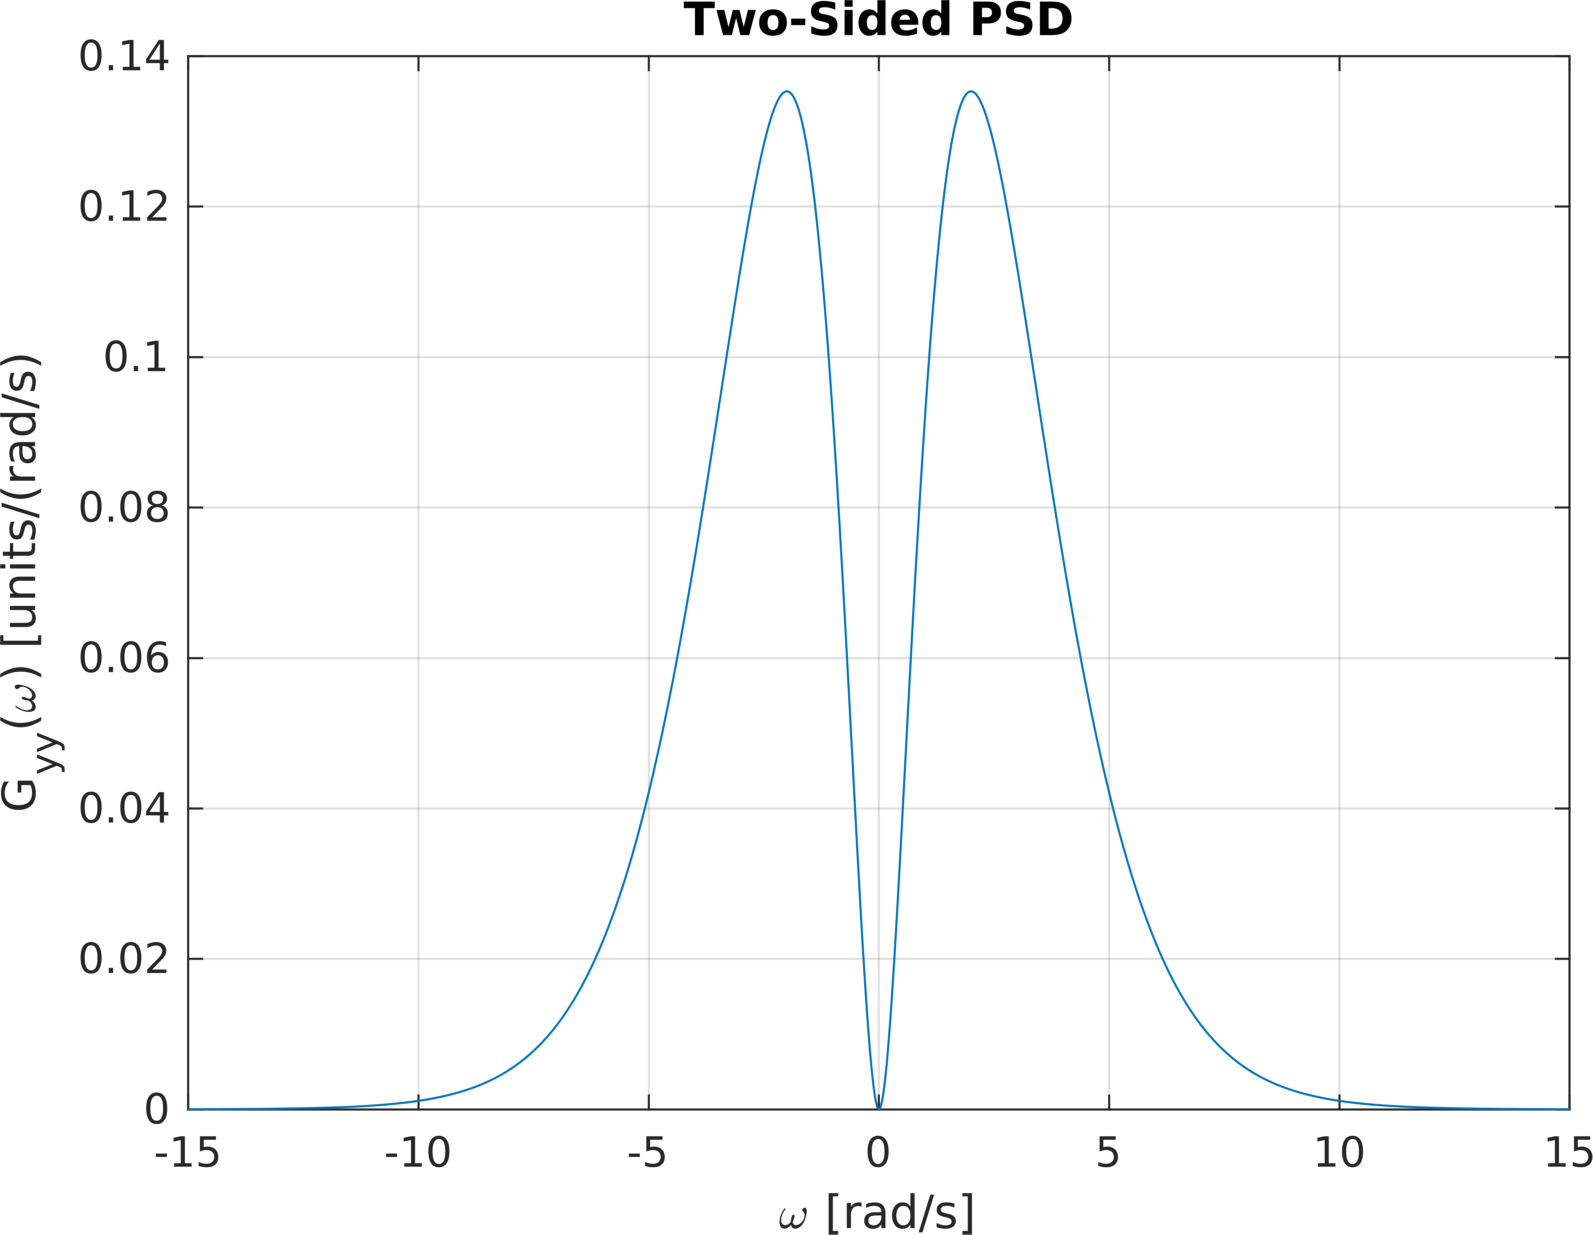
\includegraphics[width=\FigWidth\textwidth]{images/two_sided.png}
  \caption{Two-sided \ac{psd} from (\ref{e:expsd}).}
  \label{f:psd}
\end{figure}
We choose the maximum frequency for all methods to be $\omega_{max}=2\omega_u$ and choose $N=M=2^{12}$ which results in a $T_0 = \unit[1024]{s}$ and $\Delta t = \unit[0.25]{rad/s}$.  We generate a series of $M$ random phase values, $\phi^{(i)}_n$ for use in all methods.

When implementing the DTFS method (\ref{e:scfft}) with an FFT algorithm, it is important to be explicitly in the FFT implementation description because there can be differences in the conventions used when expressing (\ref{e:dft}).  The MATLAB \texttt{fft()} implementation corresponds to the convention in (\ref{e:fft}) terms of scaling and the sign of the imaginary exponential\footnote{\url{https://www.mathworks.com/help/signal/ug/discrete-fourier-transform.html}}.  To make use of the FFT convention, we express the series $B_n$ with negative imaginary values
\begin{equation}
  \beta_n = \sqrt{2} A_n e^{-j\phi^{(i)}_n}, \; n=0,1,...,M-1
\end{equation}
which allows us to use MATLAB's FFT of the $\beta_n$ series.

We implement both the sum of cosines and FFT methods for generating the sample function with the same time/frequency samples sizes of $N=M$ and the same set of $M$ random phase values.  The resulting time series, on of infinitely many sample functions, is show in Figure~\ref{f:timeseries}. 
\begin{figure}[hbt!]
  \centering
  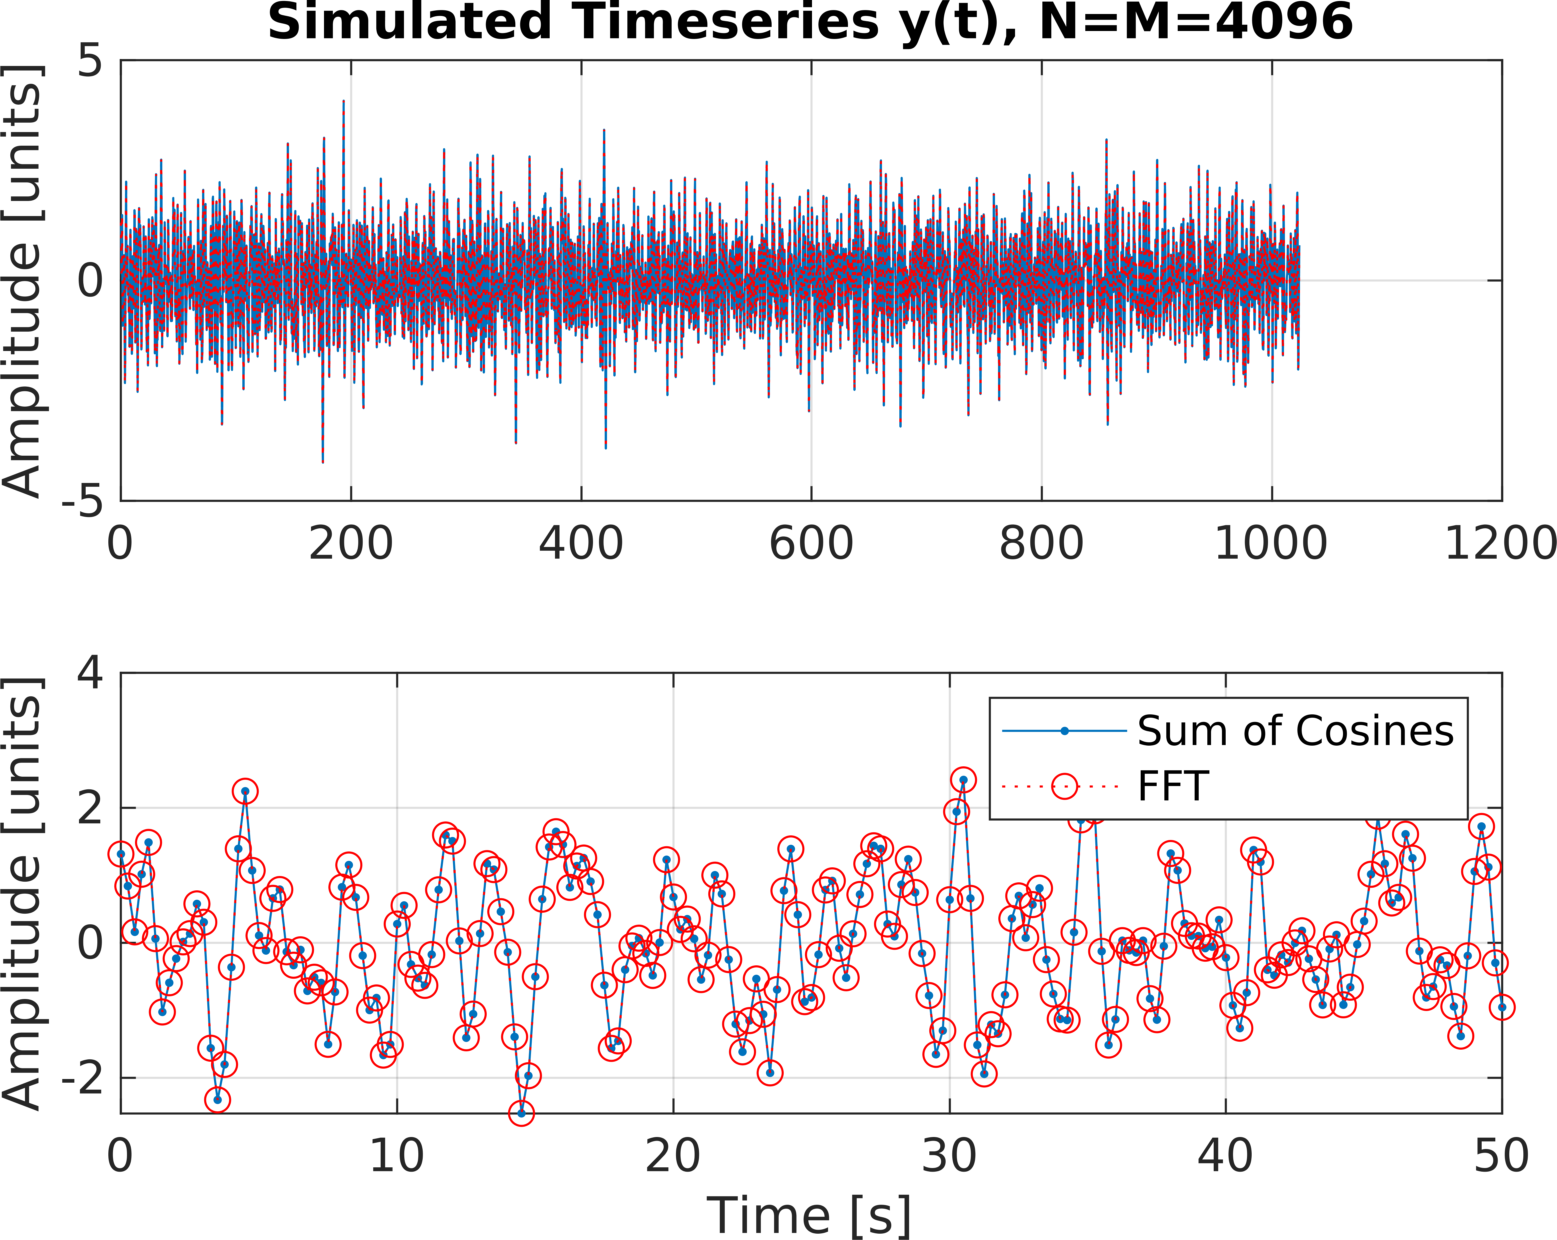
\includegraphics[width=\FigWidth\textwidth]{images/timeseries.png}
  \caption{Two example time series generated by summation of cosines and FFT}
  \label{f:timeseries}
\end{figure}
The figure illustrates that the sample functions generated by the two methods are equivalent to within numerical precision.

To verify that the generated sample functions are consistent with the original target \ac{psd}, we estimate the \ac{psd} from each sample function based on Welch's method with 1024 point FFT, Hamming windowing and 44\% overlap.  The estimated PSDs and the original target PSD are shown in Figure~\ref{f:psdest}.  Note that the estimated PSDs are the one-sided PSDs, $\Gamma(\omega)$, while the original PSD from (\ref{e:expsd}) and Figure~\ref{f:psd} is two-sided.
\begin{figure}[hbt!]
  \centering
  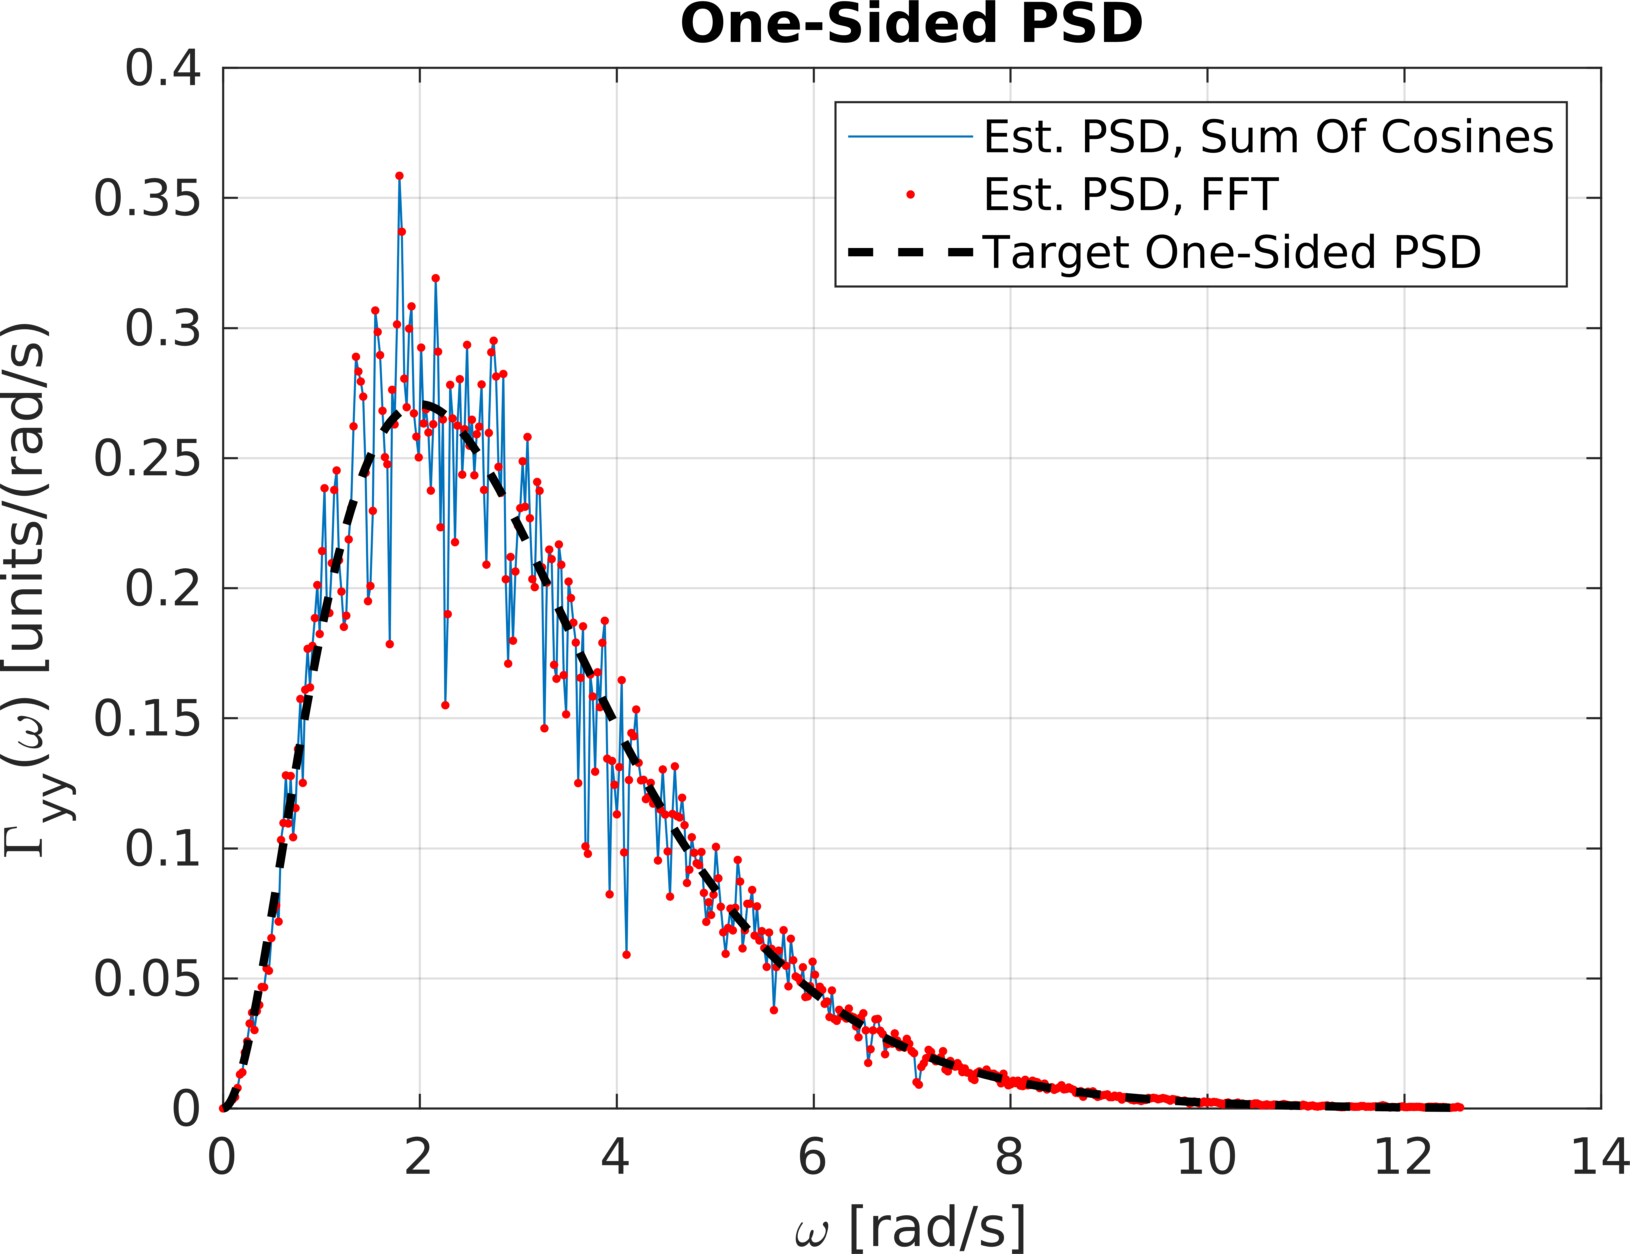
\includegraphics[width=\FigWidth\textwidth]{images/psdest.png}
  \caption{Estimates of the one-sided PSDs for the two time series from Figure~\ref{f:timeseries} shown alongside the original PSD from Figure~\ref{f:psd}. }
  \label{f:psdest}
\end{figure}
The figure illustrates that both time series have equivalent estimated PSDs and that they approximate the target PSD.  The FFT method ran $\approx 60$ times faster than the summation of cosines method: \unit[0.14]{s} vs. \unit[0.0024]{s}.  Repeating the tests various values for $M$ suggests that the speed-up ratio for the FFT method is $T_{soc}/T_{fft} = 0.04 \, M$ where $T_{soc}/T_{fft}$ is the ratio of computation time for the summation of cosines method vs. the FFT method.

The source code for this example is here: \url{https://github.com/bsb808/OceanNotes/tree/master/src/gen_timeseries_from_psd}.


\section{Conclusion}
This report documents the implementation details necessary to generate time series samples of physical processes described via an empirical \ac{psd}. It is import to maintain consistency with the scaling and conventions employed in order to generate synthetic samples statistically representative of the target phenomena.  Theses details are put into practice in MATLAB reference implementation to illustrate both summation of cosines and FFT methods to generate equivalent time series and then show that the simulated time series are statistically representative of the underlying \ac{psd}.


% REFERENCES
% List all your BibTeX reference source files (ending in *.bib extension)

% This form of the call to the bibliography:
% 1. the default thesis style, which is npsthesis.bst
% 2. assumes bib items are in the file references.bib
%\NPSbibliography{thesis}

% Please do not use a different bst (bibtex style file) to ensure formatting is correct. However, if you must risk it, it must be the first argument, and separated in []
% note: you can include multiple bib files (just comma separate them)
\NPSbibliography{bbing_master}
%\NPSbibliography{../latexlib/bib/bbing_master}

%\cleardoublepage
%\bibliographystyle{nps_thesis}
%\RaggedRight      % don't automatically full justify bibliographic references
%\singlespacing    % reduce extra line breaks between entries
%\addcontentsline{toc}{chapter}{\ULABEL\bibname}
%\bibliography{thesis}
%\doublespacing



%
% This is the official end 
%
\NPSend

% DISTRIBUTION LIST
% The list is automatically properly numbered
% and already populated with the mandatory recipients.
%
\NPSdistribution{Initial Distribution List}
\begin{distributionlist}
\item Defense Technical Information Center\\Ft. Belvoir, Virginia
\item Dudley Knox Library\\Naval Postgraduate School\\Monterey, California
%

\end{distributionlist}


\end{document}

